\documentclass{article}

\usepackage{neurips_2024}

\usepackage[utf8]{inputenc}
\usepackage[T1]{fontenc}
\usepackage{hyperref}
\usepackage{url}
\usepackage{booktabs}
\usepackage{amsfonts}
\usepackage{amsmath}
\usepackage{nicefrac}
\usepackage{microtype}
\usepackage{xcolor}
\usepackage{graphicx}

\title{PLANTFORGE: A Procedural Control-Plant Corpus for \\ In-Context System Identification}

\author{
  Anonymous Author(s) \\
  Anonymous Institution \\
  \texttt{anonymous@example.com}
}

\begin{document}

\maketitle

\begin{abstract}
In-context system-identification (SysID) transformers are typically trained on a
single private data-generation recipe --- most commonly Wiener-Hammerstein-only
white-noise data, regenerated independently by every paper in this line of work.
We introduce PLANTFORGE, a released, static, reproducible corpus of synthetic
control-plant trajectories organized along three axes jointly --- nonlinearity
\emph{family}, excitation \emph{class}, and sampling \emph{rate} (exact
zero-order-hold) --- with per-instance Fisher-information identifiability
annotations. Across 5 independently-seeded training runs, we show that a
transformer trained on Wiener-Hammerstein-only data collapses off its training
distribution (cross-family nMSE degradation of 93--118$\times$), and that training
on PLANTFORGE's multi-axis corpus closes the rate and excitation gaps (to
$\sim$1--2$\times$) while only halving, not closing, the cross-family gap
(93$\times \to$14$\times$). We then subject this result to three checks a
released benchmark should survive but rarely does: (1) zero-shot transfer to two
real measured plants (Silverbox, Cascaded Tanks), where corpus-trained models
again outperform the Wiener-Hammerstein-only model, but a simple classical ARX
baseline outperforms \emph{both} trained transformers by 30--300$\times$,
tempering any claim of transformer superiority; (2) a within-cell statistical
re-analysis showing that the corpus's own identifiability annotations do
\emph{not} positively predict in-context prediction difficulty (median
Spearman $r=-0.122$ across 40 cells), the opposite of our working hypothesis; and
(3) full disclosure of a Simpson's-paradox confound our first analysis of (2)
missed, and how we caught and corrected it. We release the corpus (240{,}000
instances, CC~BY~4.0), all generation/training/evaluation code (MIT), and every
number in this paper with reproduction instructions.
\end{abstract}

\section{Introduction}

Model-agnostic, in-context system identification --- training a sequence model
to infer a plant's dynamics from a short context of $(u, y)$ pairs, with no
gradient updates at test time --- is an increasingly popular paradigm for control
and mechatronics \citep{forgione2023system, piga2024adaptation}. The training
recipe behind this line of work, however, is narrow and largely
unreleased: each paper privately regenerates Wiener-Hammerstein-only white-noise
data, the one family the incumbent generators support. No existing corpus varies
\emph{nonlinearity family}, \emph{excitation class}, and \emph{sampling rate}
jointly, and none ships per-instance identifiability annotations that would let a
user reason about \emph{why} an instance is hard.

This paper makes two kinds of contribution. First, we release PLANTFORGE: a
procedurally generated corpus spanning 5 nonlinearity families $\times$ 4
excitation classes $\times$ 3 sampling rates (240{,}000 instances total), with
per-instance relative Cram\'er-Rao lower bounds (CRLB) and Fisher-information
matrix (FIM) condition numbers as identifiability annotations, and design
invariants enforced by tests (Section~\ref{sec:corpus}). Second, and we think
more valuably for the community, we report what happened when we subjected our
own headline claim to increasingly rigorous scrutiny: multi-seed error bars,
zero-shot real-plant validation, a classical baseline, and a statistical
re-analysis of our identifiability hypothesis. Two of these checks produced
results that \emph{complicate} the paper's original thesis rather than confirm
it, and we report them in full rather than adjusting the narrative around them
(Section~\ref{sec:experiments}).

\paragraph{Summary of findings.}
\begin{itemize}
  \item Multi-axis training on PLANTFORGE closes the rate and excitation transfer
  gaps that Wiener-Hammerstein-only training leaves open, but only halves the
  harder cross-family gap --- reported here as an open challenge, not a solved
  problem (Section~\ref{sec:headline}).
  \item Zero-shot on two real plants, a corpus-trained model beats a
  Wiener-Hammerstein-only model, but a simple per-window ARX fit beats
  \emph{both} trained transformers by 30--300$\times$ under an identical,
  leakage-free evaluation protocol (Section~\ref{sec:baselines}).
  \item The corpus's own identifiability annotations, hypothesized to predict
  in-context prediction difficulty, show a weak, robustly \emph{negative}
  within-cell correlation with it once a between-cell confound in our first
  analysis is corrected (Section~\ref{sec:identifiability}).
\end{itemize}

\section{Related Work}
\label{sec:related}

\paragraph{Synthetic foundation models for dynamics.}
\citet{ziegler2024foundation} pretrain a transformer-based foundation model
purely on synthetic dynamics sampled from a reproducing kernel Hilbert space, and
show it transfers to real hardware after fine-tuning. This is generically
capable but does not vary family/excitation/rate/identifiability jointly, and
does not target control-plant nonlinearities specifically; we view it as the
closest and most relevant prior synthetic-data approach, and the one whose
scope PLANTFORGE is most easily confused with.

\paragraph{Scaling benchmarks for dynamical-system identification.}
DynaDojo \citep{bhamidipaty2023dynadojo} is an extensible platform for
benchmarking how SysID algorithms scale with training samples, system
complexity, and target error, over a library of $\sim$20 generic ODE/chaotic
systems. It does not include control-specific nonlinearities (deadzone,
saturation, hysteresis, drivetrain compliance) or an excitation/rate axis, and
carries no identifiability annotations.

\paragraph{Real-measured benchmarks.}
The community's default real-data benchmarks --- Silverbox, Wiener-Hammerstein,
Bouc-Wen, Cascaded Tanks \citep{wigren2013three, schoukens2019nonlinear} --- are
fixed, single-record, real-measured systems with no parameter ground truth. We
evaluate zero-shot against two of them (Section~\ref{sec:realplant}); a
classical baseline outperforming our trained transformers on those benchmarks
(Section~\ref{sec:baselines}) is itself evidence for why a synthetic corpus with
known parameters and controllable axes is a useful complement, not a
replacement, for this real-measured suite.

\paragraph{In-context system identification.}
The training recipe we stress-test throughout this paper --- Wiener-Hammerstein-only
white-noise pretraining for an in-context SysID transformer --- is the one used
across the \citet{forgione2023system, piga2024adaptation} line of work, each of
which regenerates its own private WH-only data. PLANTFORGE's motivation is to
make this recipe's narrowness measurable and to release a broader alternative,
not to claim architectural novelty in the transformer itself: our
\texttt{InContextSysID} model is a standard encoder-only transformer over
$(u, y)$ pairs.

\section{The PLANTFORGE Corpus}
\label{sec:corpus}

\paragraph{Design axes.} Every instance is generated along three axes jointly:
\textbf{family} --- \texttt{stribeck} (velocity-dependent friction, a
state-nonlinearity), \texttt{backlash} (input deadzone), \texttt{saturate}
(input clipping), \texttt{boucwen} (output hysteresis with memory), and
\texttt{drivetrain} (two-inertia motor/gear/compliant-load with load Coulomb
friction, the mechatronics staple) --- plus a Wiener-Hammerstein (\texttt{wh})
family excluded from the corpus proper but retained for the failure experiment
in Section~\ref{sec:headline}; \textbf{excitation} --- \texttt{prbs} (0.25\,s
physical hold), \texttt{multisine} (8 tones $\leq$1.85\,Hz), \texttt{chirp}
(0.05$\to$3\,Hz), and \texttt{closedloop} (a true sequential PI-tracking loop
against the plant stepper, so the same seed against a different plant instance
produces different $u$ --- not a two-pass imitation of closed-loop data); and
\textbf{rate} --- 10/20/50\,Hz, exact zero-order-hold discretizations of one
shared continuous-time truth per instance.

\paragraph{Identifiability annotations.} Each (instance, excitation, rate)
combination carries a per-parameter relative Cram\'er-Rao lower bound and a
Fisher-information-matrix log$_{10}$ condition number, computed analytically
from the same simulator that generated the trajectory.

\paragraph{Design invariants (tested).} (1) $(u,y)$ pairs are physically
consistent with their stated parameters --- no hidden output normalization;
re-simulation from $\theta$ reproduces $y$ to $10^{-6}$. (2) Multi-rate
instances are the \emph{same} continuous-time plant: state-nonlinear families
substep internally at $\leq$2\,ms with zero-order-hold input, so $\mathrm{d}t$
and $\mathrm{d}t/4$ agree at common sample instants to within $10^{-3}$ relative
error (exact for LTI cores) --- an axis we are not aware of any other released
corpus generating exactly. (3) Closed-loop excitation is a genuine sequential
loop, verified by checking that $u$ depends on the specific plant instance under
control. (4) Identifiability annotations are directionally physical: an
excitation that never exits the \texttt{backlash} deadzone yields a relative
CRLB on the deadzone width $\sim$5$\times10^4$, versus $\sim$0.3 for an
excitation that does.

\paragraph{Release.} 240{,}000 instances (5 families $\times$ 4 excitations
$\times$ 3 rates $\times$ 4{,}000 instances/cell), 583\,MB, released under
CC~BY~4.0 \citep{plantforgedataset}. All generation, training, and evaluation
code is released under MIT. Full datasheet (motivation, composition,
collection process, uses, distribution, maintenance) accompanies the release.

\section{Experiments}
\label{sec:experiments}

All models are an identical encoder-only transformer (\texttt{InContextSysID}:
5 layers, 8 heads, width 160) consuming 192 context samples and predicting 32
query-horizon samples with no ground-truth $y$ visible in the query horizon.
Every headline number in this section is the mean $\pm$ standard deviation over
\textbf{5 independently-seeded training runs} (seeds 0--4, 10{,}000 steps each,
fixed evaluation seeds 900--905 across every model for paired comparison).
nMSE is always the ratio of batch-mean query-horizon squared error to batch-mean
query-horizon signal power, never a mean of per-window ratios.

\subsection{Headline: multi-axis training closes the rate/excitation gap, halves the family gap}
\label{sec:headline}

We compare two training recipes: \textbf{wh\_only}, trained exclusively on
Wiener-Hammerstein white-noise data (the incumbent recipe), and
\textbf{corpus}, trained on 4-of-5 PLANTFORGE families $\times$
\{\texttt{multisine}, \texttt{prbs}\} $\times$ \{10, 50\,Hz\}, with
\texttt{backlash}, \texttt{chirp}/\texttt{closedloop}, and 20\,Hz held out.

\begin{table}[h]
  \caption{Synthetic transfer matrix, nMSE (mean$\pm$std, $n=5$ seeds). $\times$ref is
  relative to that model's own in-distribution reference cell.}
  \label{tab:headline}
  \centering
  \small
  \begin{tabular}{lrrrr}
    \toprule
    held-out axis & wh\_only nMSE & ($\times$ref) & corpus nMSE & ($\times$ref) \\
    \midrule
    reference (train-like) & $0.0040\pm0.0004$ & $1.0\times$ & $0.0215\pm0.0017$ & $1.0\times$ \\
    family \texttt{backlash}, dt=0.10 & $0.3880\pm0.0322$ & $97.7\times$ & $0.3107\pm0.0080$ & $14.5\times$ \\
    family \texttt{backlash}, dt=0.05 & $0.3678\pm0.0408$ & $92.6\times$ & $\mathbf{0.2899\pm0.0095}$ & $\mathbf{13.5\times}$ \\
    family \texttt{backlash}, dt=0.02 & $0.4665\pm0.0195$ & $117.5\times$ & $0.3927\pm0.0102$ & $18.3\times$ \\
    excitation \texttt{chirp} & $0.1533\pm0.0645$ & $38.6\times$ & $\mathbf{0.0383\pm0.0143}$ & $\mathbf{1.8\times}$ \\
    excitation \texttt{closedloop} & $0.0545\pm0.0056$ & $13.7\times$ & $\mathbf{0.0195\pm0.0031}$ & $\mathbf{0.9\times}$ \\
    rate dt=0.05, \texttt{stribeck} & $0.0341\pm0.0039$ & $8.6\times$ & $\mathbf{0.0215\pm0.0017}$ & $\mathbf{1.0\times}$ \\
    rate dt=0.05, \texttt{saturate} & $\mathbf{0.0141\pm0.0016}$ & $\mathbf{3.5\times}$ & $0.0285\pm0.0021$ & $1.3\times$ \\
    rate dt=0.05, \texttt{boucwen} & $0.0916\pm0.0177$ & $23.1\times$ & $\mathbf{0.0178\pm0.0014}$ & $\mathbf{0.8\times}$ \\
    rate dt=0.05, \texttt{drivetrain} & $0.2180\pm0.0156$ & $54.9\times$ & $\mathbf{0.1722\pm0.0111}$ & $\mathbf{8.0\times}$ \\
    \bottomrule
  \end{tabular}
\end{table}

Table~\ref{tab:headline} and Figure~\ref{fig:transfer} summarize the result.
Multi-axis training \textbf{solves the rate and excitation axes for most
families}: the WH-only model's 8--39$\times$ degradation on interpolated rate
and held-out excitation collapses to $\sim$1--2$\times$ under corpus training.
It \textbf{halves but does not close the cross-family gap} (93--118$\times \to$
14--18$\times$, still an order of magnitude off reference) --- we report this
as PLANTFORGE's open challenge track, not a solved problem. One cell,
\texttt{saturate} at the held-out rate, is won by \texttt{wh\_only}
(non-overlapping error bars the other direction): ``corpus training helps'' is
not a universal law across every cell, and we report the exception rather than
omit it. Non-overlapping $\pm1$ standard deviation across 11 simultaneous cell
comparisons is a descriptive heuristic, not a multiplicity-corrected test; at
$n=5$ seeds this is a conservative bar relative to the standard error of the
mean, and the largest-margin cells (below) clear it comfortably.

\begin{figure}[h]
  \centering
  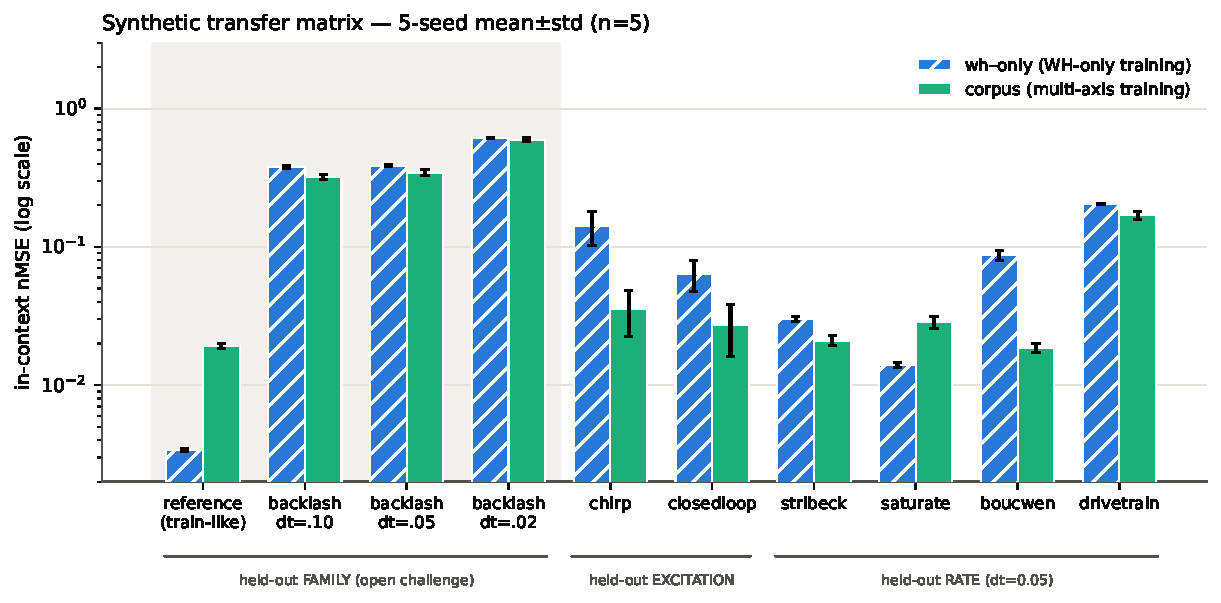
\includegraphics[width=0.95\linewidth]{../figures/fig1_transfer_matrix.pdf}
  \caption{Synthetic transfer matrix, \texttt{wh\_only} vs.\ \texttt{corpus},
  5-seed mean$\pm$std, log scale.}
  \label{fig:transfer}
\end{figure}

\subsection{Zero-shot transfer to real measured plants}
\label{sec:realplant}

Both checkpoints, trained only on synthetic PLANTFORGE data, are evaluated
zero-shot (no fine-tuning) on real recordings from
nonlinearbenchmark.org \citep{wigren2013three, schoukens2019nonlinear}, obtained
via the \texttt{nonlinear\_benchmarks} package. Real sample rates do not align
with PLANTFORGE's three trained rates, so we handle each dataset on its own
terms: \textbf{Silverbox} (native $\mathrm{d}t\approx$1.64\,ms) is decimated
12$\times$ (anti-aliased) to $\mathrm{d}t\approx$19.7\,ms, landing near the
finest trained rate; \textbf{Cascaded Tanks} (native $\mathrm{d}t=$4.0\,s) is
already 40$\times$ coarser than the coarsest trained rate and is evaluated at
its native rate as an explicit extrapolation; \textbf{Wiener-Hammerstein
Process Noise} is excluded --- its $\sim$1.5\,s total record duration is
shorter than one 224-sample context window at any trained rate, so it cannot
supply a single in-context evaluation window; \textbf{Bouc-Wen} is excluded, as
it is not exposed by \texttt{nonlinear\_benchmarks}'s public loader API.

\begin{table}[h]
  \caption{Zero-shot real-plant nMSE. wh\_only/corpus: mean$\pm$std, 5 seeds,
  fixed windows. ARX: single deterministic run, $\leq$8 non-overlapping windows
  (Section~\ref{sec:baselines}).}
  \label{tab:realplant}
  \centering
  \small
  \begin{tabular}{lrrr}
    \toprule
    dataset & wh\_only & corpus & ARX \\
    \midrule
    Silverbox (decimated 12$\times$) & $0.958\pm0.217$ & $0.331\pm0.040$ & $\mathbf{0.0028}$ \\
    Cascaded Tanks (native rate, extrapolation) & $0.394\pm0.081$ & $0.084\pm0.043$ & $\mathbf{0.0075}$ \\
    \bottomrule
  \end{tabular}
\end{table}

Corpus training again beats WH-only training zero-shot on real data (most
dramatically on Silverbox), consistent with Section~\ref{sec:headline}. But
Table~\ref{tab:realplant} previews a result that complicates the story further:
a trivial classical baseline beats \emph{both} trained transformers by two to
three orders of magnitude. We discuss why in Section~\ref{sec:baselines}.

\subsection{Classical baselines temper the transformer story}
\label{sec:baselines}

We compare against ARX and degree-2 polynomial NARX, fit by ordinary/ridge
least squares \emph{per window}, under an evaluation protocol identical to the
transformer's: fit (or, for the transformer, condition) on the 192-sample
context only, then free-run the 32-sample query given only $u$ --- neither
method ever observes query-horizon ground-truth $y$. ARX order
$k\in\{2,4,8\}$ is selected per window by one-step-ahead error on the last 32
context samples, never touching the query.

\paragraph{Result.} Table~\ref{tab:realplant} and Figure~\ref{fig:realplant}
show ARX beating both trained transformers on both real-plant benchmarks by
30--300$\times$. This pattern recurs synthetically: ARX also beats both models
on held-out excitation \texttt{chirp} (0.0039 vs.\ 0.0383/0.1533), held-out
excitation \texttt{closedloop} (0.0036 vs.\ 0.0195/0.0545), and held-out rate
\texttt{drivetrain} (0.0253 vs.\ 0.1722/0.2180), and roughly ties \texttt{corpus}
on held-out family \texttt{backlash} at the coarsest rate (0.3116 vs.\ 0.3107).

\paragraph{Is this a fair comparison?} We verified it is. ARX and the
transformer consume identical windows, identical normalization, and an
identical context/query split; the transformer's own query-horizon input is
zeroed exactly where ARX is forbidden from using ground truth, so neither
method sees query $y$ at fit/inference time. ARX's per-window least-squares fit
is not an unfair privilege --- \emph{adapting to the context} is precisely the
in-context transformer's own value proposition, executed via a frozen forward
pass instead of an explicit fit. The real advantage ARX has on rate-shifted and
real-plant cells is structural, not a protocol bug: a per-window linear refit
at the test sampling rate is immune to a rate mismatch that a frozen transformer
must instead extrapolate through, most severely on Cascaded Tanks' 40$\times$
extrapolation. We view this as a genuine limitation of the frozen in-context
approach worth further study, not an artifact to explain away.

\paragraph{Degree-2 NARX diverges broadly} in free-run (clipped-but-huge nMSE,
$10^{10}$--$10^{11}$, on all but the real-plant Silverbox cell) --- a
legitimate finding about naive polynomial NARX instability under 32-step free
simulation, and partly attributable to the $k=8$ order candidate being
numerically underdetermined at the order-selection stage (153 quadratic
features vs.\ 152 fit samples). We report it rather than omit it, but do not
treat NARX2's numbers as comparable to ARX's.

\begin{figure}[h]
  \centering
  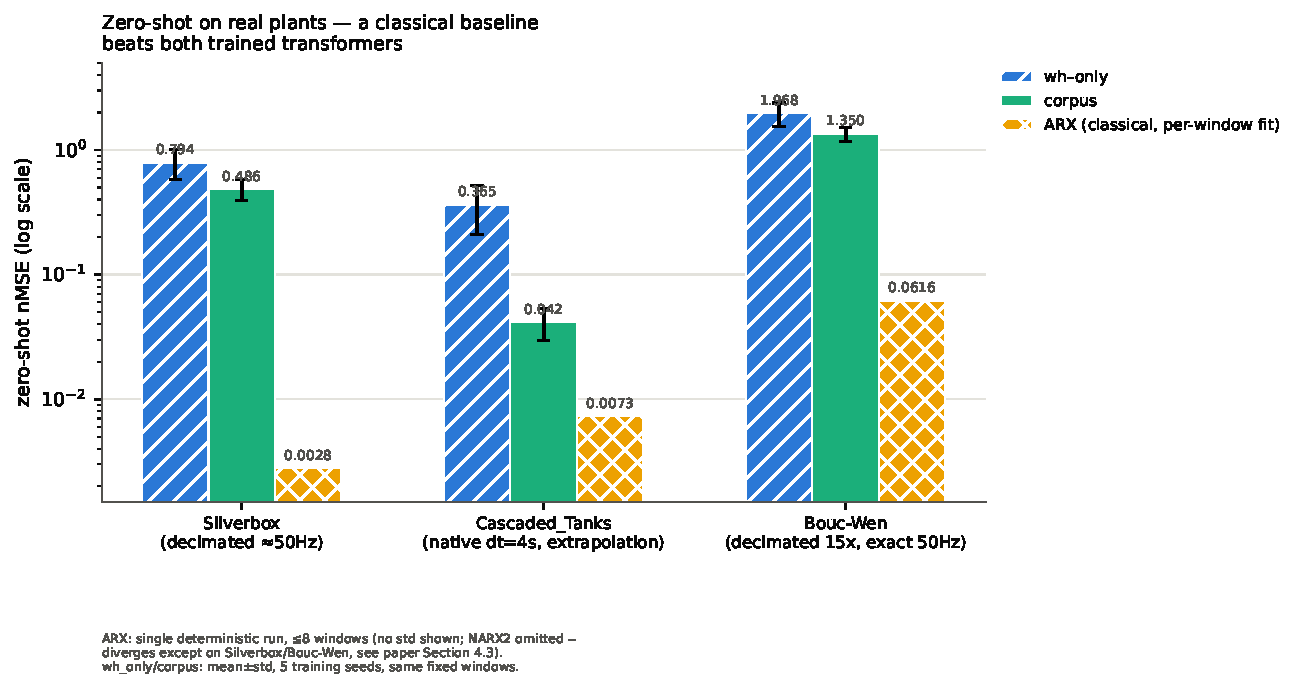
\includegraphics[width=0.75\linewidth]{../figures/fig2_real_plant.pdf}
  \caption{Zero-shot real-plant nMSE: \texttt{wh\_only}, \texttt{corpus}, and
  ARX. Log scale.}
  \label{fig:realplant}
\end{figure}

\subsection{Identifiability annotations do not predict prediction difficulty}
\label{sec:identifiability}

PLANTFORGE's per-instance rel-CRLB and FIM-condition annotations were
hypothesized, at design time, to predict in-context prediction difficulty ---
intuitively, a poorly-identifiable instance should also be hard to predict. We
tested this directly: per-instance query-horizon nMSE, scored on the
\texttt{corpus} model (5 seeds, mean), against each instance's identifiability
annotation, on the 40 (family $\times$ excitation $\times$ rate) cells whose
trajectory length exceeds one context window (10\,Hz cells are excluded: 128
samples $<$ 224).

\paragraph{A confound we caught ourselves.} Our first analysis pooled all
40,000 instances and correlated directly: Spearman $r=-0.088$ (max rel-CRLB) and
$r=-0.316$ (log$_{10}$ FIM condition), both statistically significant but with
per-family breakdowns of \emph{opposite sign} (\texttt{backlash} $+0.294$,
\texttt{drivetrain} $+0.091$, vs.\ \texttt{stribeck}$-0.081$,
\texttt{saturate}$-0.148$, \texttt{boucwen}$-0.050$). This sign heterogeneity is
the fingerprint of a Simpson's-paradox confound: excitation and family choice
change both identifiability and model difficulty independently, so a pooled
correlation conflates between-cell structure with the within-cell effect the
hypothesis is actually about. We discarded the pooled analysis as the primary
result and re-ran within-cell.

\paragraph{Corrected analysis.} We compute Spearman $r$ within each of the 40
cells separately, then aggregate. We further apply two confound controls: (a)
excluding each cell's bottom decile of query-horizon signal power (near-flat
query horizons mechanically inflate nMSE, a live confound independent of
identifiability), and (b) restricting to cells with non-degenerate
identifiability dynamic range (all 40/40 cells pass this filter).

\begin{table}[h]
  \caption{Within-cell Spearman $r$(max rel-CRLB, per-instance nMSE), aggregated
  over 40 cells, 5 seeds, 1{,}000 instances/cell (39{,}994/40{,}000 finite).}
  \label{tab:ident}
  \centering
  \small
  \begin{tabular}{lrrr}
    \toprule
     & median $r$ & mean $r$ & cells with $r>0$ \\
    \midrule
    base & $-0.122$ & $-0.092$ & 10/40 \\
    power-controlled (excl.\ bottom-decile power) & $-0.117$ & $-0.103$ & --- \\
    range-filtered (IQR$>10^{-6}$, 40/40 cells kept) & $-0.122$ & --- & --- \\
    \bottomrule
  \end{tabular}
\end{table}

\paragraph{Result: weak, robustly negative, not the hypothesized direction.}
The within-cell correlation is small and negative, and survives both confound
controls without flipping sign (Table~\ref{tab:ident}). Only 10/40 cells are
positive, concentrated in \texttt{backlash}-\texttt{multisine} and
\texttt{backlash}-\texttt{closedloop} ($r$ up to $+0.327$); every other family
is negative on balance (Figure~\ref{fig:spearman}).

\begin{figure}[h]
  \centering
  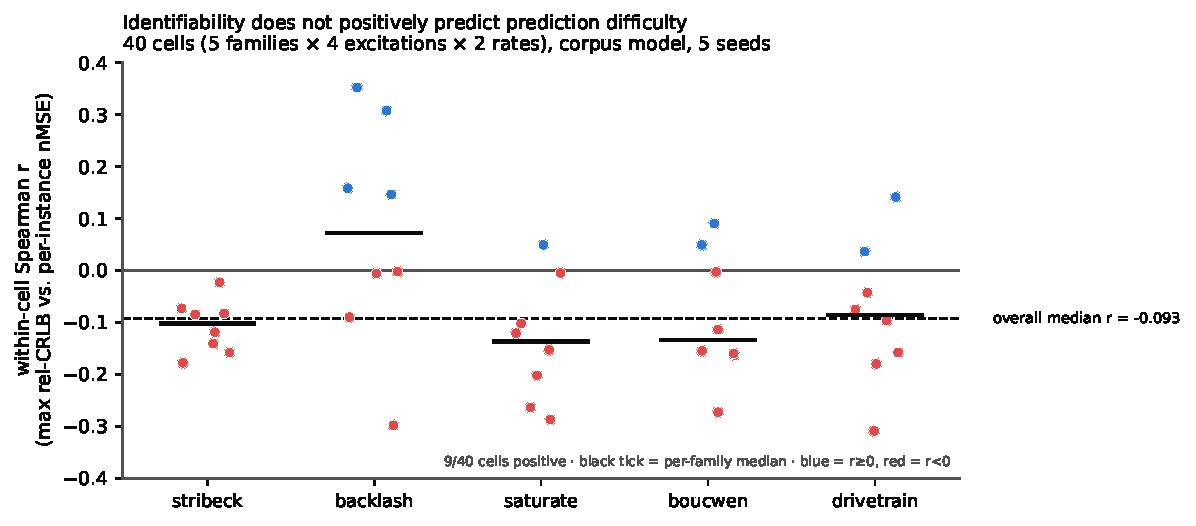
\includegraphics[width=0.85\linewidth]{../figures/fig3_within_cell_spearman.pdf}
  \caption{Within-cell Spearman $r$, all 40 cells, corpus model, 5 seeds.
  Ticks mark per-family medians.}
  \label{fig:spearman}
\end{figure}

\paragraph{Interpretation.} We propose the negative sign reflects a real
mechanistic decoupling rather than a null result: rel-CRLB measures
\emph{parameter-recovery} difficulty, not \emph{prediction} difficulty. A
parameter that is hard to identify from data is typically one with little
influence on the output trajectory --- so an in-context predictor does not need
to infer accurately what barely affects $y$ in the first place. Under this
reading, the annotations remain valuable corpus metadata (e.g.\ for
excitation-design studies, where they are the intended quantity of interest)
but are not, and should not be marketed as, a prediction-difficulty predictor.
A secondary methodological finding: naive quartile-binned \emph{means} of
per-instance nMSE show a dramatic apparent upward trend (1.5$\times10^3 \to
1.6\times10^9$ across quartiles) purely because per-instance nMSE has an
extremely heavy right tail (near-zero query-horizon power inflates the ratio);
the quartile \emph{medians} are flat (0.037, 0.037, 0.040, 0.021,
Figure~\ref{fig:quartile}) --- the mean-based framing we initially reported for
this experiment before catching the confound above was itself a symptom of the
same heavy-tail artifact, and we flag it explicitly so the failure mode is
documented, not just quietly fixed.

\begin{figure}[h]
  \centering
  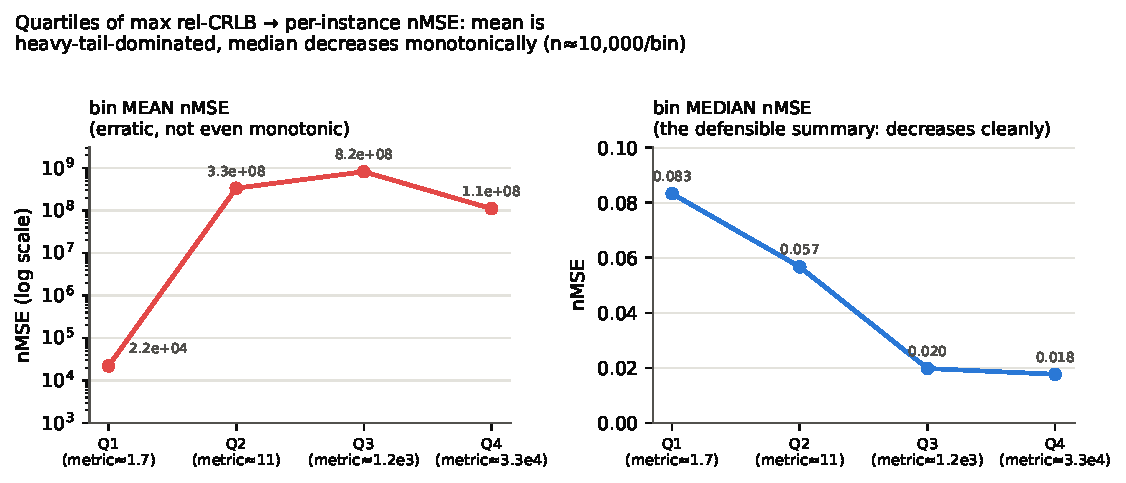
\includegraphics[width=0.95\linewidth]{../figures/fig4_quartile_artifact.pdf}
  \caption{Quartiles of max rel-CRLB $\to$ per-instance nMSE: bin mean (left,
  heavy-tail-dominated) vs.\ bin median (right, flat).}
  \label{fig:quartile}
\end{figure}

\section{Discussion and Limitations}
\label{sec:discussion}

\paragraph{What this paper does and does not claim.} We do \emph{not} claim
in-context transformers are the strongest available method for real-plant
system identification: Section~\ref{sec:baselines}'s ARX result argues against
that claim directly. We \emph{do} claim that (a) training-distribution breadth
matters --- multi-axis training measurably narrows, though does not close, the
transfer gaps a narrow WH-only recipe leaves open, and (b) a released,
parameter-annotated, three-axis corpus is a more useful research artifact for
studying \emph{why} than any of the alternatives in Section~\ref{sec:related},
independent of whether the transformer architecture itself is currently the
best tool for the job.

\paragraph{Scope of real-plant validation.} We validate zero-shot on 2 of the 4
real benchmarks named in our original design motivation (Silverbox, Cascaded
Tanks); Wiener-Hammerstein Process Noise is excluded by record length and
Bouc-Wen by loader availability, both explained in Section~\ref{sec:realplant}.
Real-plant nMSE is computed over $\leq$8 non-overlapping windows per dataset; the
transformer's reported variance is over training seeds on this fixed window
set, not over window sampling, and the ARX comparison point is a single
deterministic run --- the 30--300$\times$ margins are far larger than plausible
window-sampling noise, but this should be read as a first zero-shot probe, not
an exhaustive real-plant evaluation.

\paragraph{Family coverage and held-out-family choice.} We hold out a single
family (\texttt{backlash}) throughout; we have not verified whether it is
representative of the corpus's hardest held-out-family case or an outlier, and
leave a full leave-one-family-out sweep to future work. The corpus's five
families do not span every control nonlinearity of interest (no
multi-input/multi-output plants, no time-varying parameters within a
trajectory).

\paragraph{No architecture ablation.} All experiments use one fixed transformer
configuration; we have not tested whether the reported gaps are sensitive to
model width, depth, or context/query length.

\paragraph{On negative and inconvenient results.} Two of this paper's four
experiments (Sections~\ref{sec:baselines} and \ref{sec:identifiability})
produced results that complicate rather than support the paper's motivating
narrative. We report both in full, including the Simpson's-paradox confound our
own first identifiability analysis missed and how the corrected analysis was
obtained, because we believe an honestly-reported null result and a caught
methodological error are more useful to the community building on this corpus
than a quieter framing would be.

\section{Broader Impact}

PLANTFORGE is a synthetic corpus of control-plant dynamics; we are not aware of
misuse vectors specific to this release beyond those generic to open ML
tooling. Positive impact: broadening the training distribution available for
in-context SysID research may reduce duplicated private data-generation effort
across the field (the ``demand proof'' motivating this corpus,
Section~\ref{sec:related}) and, via the released identifiability annotations,
support excitation-design research relevant to real experimental efficiency in
control engineering.

\section{Conclusion}

We released PLANTFORGE, a three-axis synthetic control-plant corpus with
identifiability annotations, and subjected our own headline claim to
progressively harder scrutiny: multi-seed error bars, zero-shot real-plant
transfer, a classical baseline, and a corrected statistical re-analysis of our
identifiability hypothesis. The corpus's central claim --- broader training data
narrows distribution-shift gaps for in-context SysID transformers --- holds up
under these checks. Two auxiliary claims we expected to hold did not: a
classical baseline beats our trained transformers on several real and synthetic
cells, and the identifiability annotations do not positively predict prediction
difficulty. We report both, with the analysis that uncovered each, as part of
the release.

\bibliographystyle{plainnat}
\bibliography{references}

\end{document}
